%
% funktionen.tex
%
% (c) 2018 Prof Dr Andreas Müller
%
\section{Funktionenräume%
\label{section:funktionenraume}}
\index{Funktionenraum}%
\rhead{Funktionenräume}
Die abgetasteten Signale haben einen endlichdimensionalen Vektorraum
mit Skalarprodukt gebildet und darin könnte man auch bereits ein
ansprechend interessante Theorie aufbauen.
Zum Beispiel könnte man bereits eine Form der diskreten
Fourier-Transformation entwickeln, wie das zum Beispiel in
\cite{buch:mathsem-klima} geschieht.
Für die Entwicklung der Wavelettheorie ist notwendig, dass Signale
entlang der Zeitachse beliebig fein aufgelöst werden können, was
mit einem bereits abgetasteten Signal nicht möglich ist.
Es muss daher eine Theorie entwickelt werden, in der man mit
Funktionen genau gleich arbeiten kann wie mit den Vektoren von
Abtastwerten.
Insbesondere wird angestrebt, Skalarprodukte von Funktionen
zu bilden und orthonormierte Basen zu konstruieren. 
Dieses Ziel wird allerdings erst in Kapitel~\ref{chapter:fourier} erreicht werden.

\subsection{Vektorräume von Funktionen}
Sei $X$ eine Menge, dann ist
\[
\mathbb R^X = \{ f\colon X\to\mathbb R\}
\]
die Menge der Funktionen auf $X$ mit reellen Werten.
Sie kann auf natürlich Art und Weise zu einem Vektorraum gemacht werden.
Dazu müssen die Operationen Addition und Multiplikation mit Skalaren
definiert werden

\begin{definition}
Die Vektorraumoperationen auf $\mathbb R^X$ sind definiert durch
\[
\begin{aligned}
&\text{Addition:}
&
f,g&\in \mathbb R^X
	&&\Rightarrow
	&(f+g)&\colon X\to\mathbb R:x\mapsto f(x)+g(x)
\\
&\text{Multiplikation:}
&
f&\in\mathbb R^X, \lambda\in\mathbb R
	&&\Rightarrow
	&(\lambda f)&\colon X\to\mathbb R:x\mapsto \lambda f(x)
\end{aligned}
\]
\end{definition}

\begin{beispiel}
Für $X=\{1,\dots,N\}$ ist $f\in \mathbb R^X$ gleichbedeutend mit
der Vorgabe der Funktionswerte $(f(1),\dots,f(N))$.
Diese können auch als Spaltenvektoren
\[
\vec{f} = \begin{pmatrix}f(1)\\\vdots\\f(N)\end{pmatrix}
\]
geschrieben werden.
Die Rechenoperationen in $\mathbb R^X$ und $\mathbb R^N$ sind gleichbedeutend,
wie man zum Beispiel für die Addition verifizieren kann:
\[
\overrightarrow{(f+g)}
=
\begin{pmatrix}
(f+g)(x_1)\\\vdots\\(f+g)(x_N)
\end{pmatrix}
=
\begin{pmatrix}
f(x_1)+g(x_1)\\\vdots\\f(x_N)+g(x_N)
\end{pmatrix}
=
\begin{pmatrix}
f(x_1)\\\vdots\\f(x_N)
\end{pmatrix}
+
\begin{pmatrix}
g(x_1)\\\vdots\\g(x_N)
\end{pmatrix}
=
\vec{f} + \vec{g}.
\]
$\mathbb R^X$ ist also nur eine neue Schreibweise für den altbekannten
Vektorraum $\mathbb R^N$.
\end{beispiel}

Die Konstruktion wird interessant, wenn $X$ zusätzliche Struktur hat.
Wenn $X$ eine Teilmenge von $\mathbb R^n$ ist, dann kann man sich auf
stetige Funktionen beschränken und daraus einen Vektorraum bauen.

\begin{definition}
Ist $X\subset\mathbb R^n$, dann wird die Menge der stetigen reellwertigen
\index{$C(X,\mathbb R)$}%
\index{stetige Funktion}%
Funktionen auf $X$ mit
\[
C_{\mathbb R}(X)
=
C(X,\mathbb R)
=
\{ f\in \mathbb R^X\,|\,\text{$f$ ist stetig}\}
\]
bezeichnet.
\end{definition}

Diese Definition ist kompatibel mit den Vektoraumoperationen,
denn in der Analysis lernt man, dass eine Linearkombination
stetiger Funktionen wieder stetig ist.

Man kann sogar einen Begriff des Abstands zwischen zwei Funktionen
definieren mit Hilfe der {\em Norm}:

\begin{definition}
Die {\em Supremumnorm} einer Funktion $f\in C(X,\mathbb R)$ ist
\index{Supremumnorm}%
\[
\|f\| = \sup_{x\in X} |f(x)|.
\]
Um die Supremumnorm von anderen Normen zu unterscheiden, wird sie
manchmal auch $\|f\|_{\infty}$ geschrieben.
\end{definition}

Man beachte aber, dass diese Art von Norm von grundsätzlich anderer Art
ist wie der geometrische Abstandsbegriff.
Dank der Pythagoras-Formel wirkt sich jede Koordinate eines Vektors 
auf die übliche geometrische Norm aus.
In der Supremumnorm spielt nur der maximale Wert eine Rolle,
Änderungen an kleineren Funktionswerten verändern den Abstand nicht.

Von besonderem Interesse ist für die Zwecke der Signalanalyse und
-synthese natürlich der Definitionsbereich $X=\mathbb{R}$, der
zusätzliche algebraische, geometrische und analytische Struktur trägt, die man
zur Definition einer Norm verwenden kann, wie wir später sehen werden.

\subsection{Translation und Dilatation\label{subsection:translation-dilatation}}
Der Definitionsbereich $\mathbb R$ zeichnet sich durch die darin zur
Verfügung stehenden Rechenoperationen aus.
Man kann zu einem Argument einen konstanten Wert hinzuaddieren oder mit
einer Zahl multiplizieren, bevor man eine Funktion auswertet.
Daraus ergeben sich die zwei Operationen der Translation und der Dilatation.
\index{Translation}%
\index{Dilatation}%

\begin{figure}
\centering
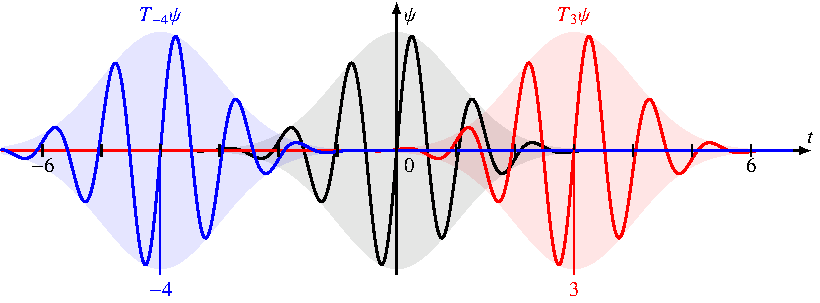
\includegraphics[width=\hsize]{chapters/1-geometrie/images/translation.pdf}
\caption{Wirkung des Operators $T_b$ auf das Gabor-Wavelet
$\psi(t) = e^{-t^2/2}\sin(6t)$,
der Graph von $T_b\psi$ ist um $b$ nach rechts verschoben.
\label{geometrie:Tb:image}}
\end{figure}
\begin{figure}
\centering
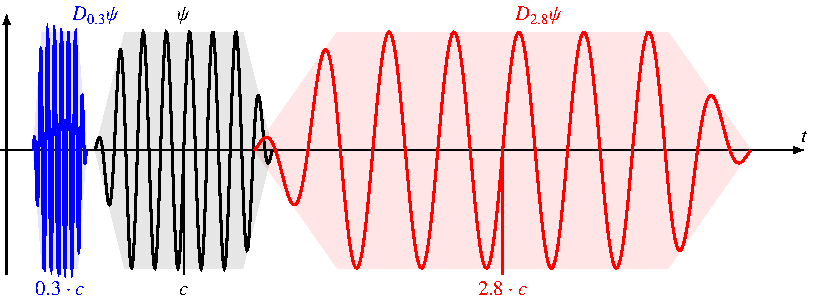
\includegraphics[width=\hsize]{chapters/1-geometrie/images/dilatation.pdf}
\caption{Wirkung des Operators $\tilde{D}_a$ auf ein im Punkt $c$ zentriertes
Wavelet $\psi$. Das Wavelet $\tilde{D}_a\psi$ ist zentriert im Punkt $a\cdot c$.
\label{geometrie:Da:image}}
\end{figure}

\begin{definition}
Sei $f$ eine Funktion auf $\mathbb R$ mit Werten in $Y$.
Dann setzt man
\begin{align*}
T_bf&\colon \mathbb R \to Y: t\mapsto f(t-b)&&\text{Translation}
\\
\tilde{D}_af&\colon \mathbb R \to Y: t\mapsto f(t/a)&&\text{Dilatation}
\end{align*}
\end{definition}

Die Wirkung der beiden Operatoren ist in den
Abbildungen~\ref{geometrie:Tb:image} und \ref{geometrie:Da:image} dargestellt.
Der Operator $\tilde{D}_a$ dehnt den Graphen der Funktion entlang der
$t$-Achse um den Faktor $a$ während der Operator $T_b$ den Graphen
der Funktion um den Betrag $b$ entlang der $t$-Achse verschiebt.

Die gewählte Notation für die Dilatation ist etwas asymmetrisch.
Der Grund ist, dass Operation $T_b$ die später zu definierende,
skalarproduktbasierte Norm erhält, dass aber $\tilde{D}_a$ diese Norm
verändert.
Die später formulierte Definition von $D_a$ wird erreichen, dass 
die $D_a$ die zum Skalarprodukt gehörige Norm erhält.

\begin{satz}
\label{geometrie:satz:inverse}
Die Operatoren $T_b$ und $\tilde{D}_a$ sind invertierbar und es gilt
\[
T_b^{-1} = T_{-b}
\qquad\text{und}\qquad
\tilde{D}_a^{-1} = \tilde{D}_{1/a}.
\]
\end{satz}

\begin{proof}[Beweis]
Die folgenden Rechnungen zeigen, dass $T_bT_{-b}f=f$ und $\tilde{D}_a\tilde{D}_{1/a}f=f$:
\begin{align*}
(T_bT_{-b}f)(t)
&=
(T_{-b})f(t-b)
=
f((t+b)-b)
=
f(t)
\\
(\tilde{D}_a\tilde{D}_{1/a}f)(t)
&=
(\tilde{D}_{1/a}f)(t/a)
=
f((t/{\textstyle\frac1a})/a)
=
f(t).
\qedhere
\end{align*}
\end{proof}

\begin{figure}
\centering
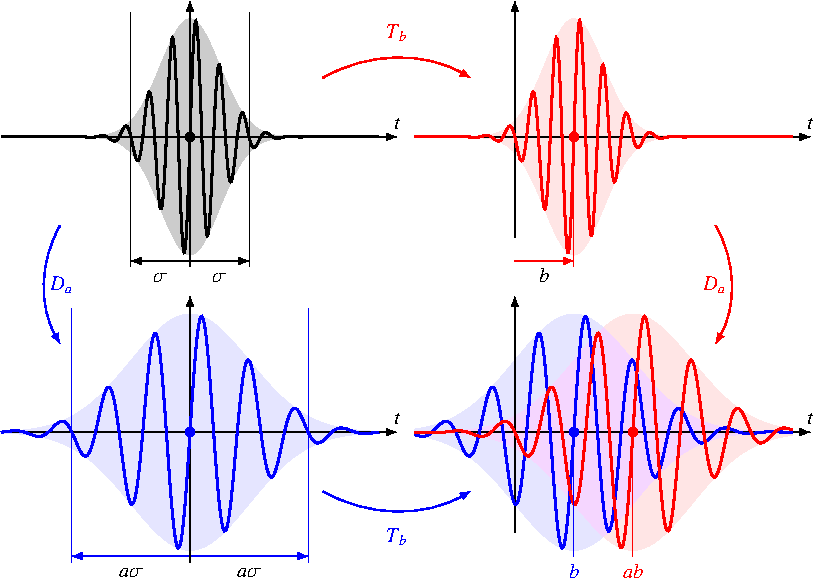
\includegraphics[width=\hsize]{chapters/1-geometrie/images/kommutator.pdf}
\caption{Die Operatoren $T_b$ und $D_a$ vertauschen nicht.
Der rote Pfad wendet erst $T_b$ und dann $D_a$ an, der blaue zuerst
$D_a$ und dann erst $T_b$.
In beiden Fällen erhält man ein um den Faktor $a$ gestrecktes
Wellenpaket.
Im Fall $T_b\circ D_a$ erhält man ein im Punkt $b$ zentriertes Wellenpaket
(blaue), während es im Falle $D_a\circ T_b$ im Punkt $ab$ zentriert ist (rot).
Wendet man in der unteren Zeile statt $T_b$ den Operator $T_{ab}$ an, 
kommen die beiden Wellenpakete zur Deckung, was die Vertauschungsregel
von Satz~\ref{satz:kommutator} bestätigt.
\label{geometrie:kommutator:image}}
\end{figure}

\begin{satz}
\label{satz:kommutator}
Translation $T_b$ und Dilatation $\tilde{D}_a$ sind lineare Abbildungen.
Die beiden Operatoren vertauschen nicht, vielmehr gilt
$T_{ab}\tilde{D}_a = \tilde{D}_aT_b$.
\end{satz}
\index{Vertauschungsregel für $T_b$ und $D_a$}%

\begin{proof}[Beweis]
Die Linearität der Operatoren wird durch Nachrechnen verifiziert.
Für eine Linearkombination $\lambda f+\mu g$ zweier Funktionen $f$ und $g$ gilt:
\begin{align*}
\tilde{D}_a(\lambda f+\mu g)(t)
&=
(\lambda f+\mu g)(t/a)
=
\lambda f(t/a)+\mu g(t/a)
=
\lambda (\tilde{D}_af)(t)+\mu (\tilde{D}_ag)(t),
\\
T_b(\lambda f+ \mu g)(t)
&=
(\lambda f+\mu g)(t-b)
=
\lambda f(t-b)+\mu g(t-b)
=
\lambda (T_bf)(t)+\mu (T_bg)(t).
\end{align*}
Ohne Argumente geschrieben heisst dies
\begin{align*}
\tilde{D}_a(\lambda f+\mu g) &= \lambda \tilde{D}_af + \mu \tilde{D}_ag,
\\
T_b(\lambda f+\mu g) &= \lambda T_bf + \mu T_bg.
\end{align*}
Damit ist die Linearität bewiesen.

Für die Vertauschungsregel müssen die beiden Seiten der Regel
berechnet werden.
Die Wirkung der beiden Operatoren in verschiedener Reihenfolge
ist:
\begin{align*}
(T_bf)(t)
&=
f(t-b),
\\
(\tilde{D}_af)(t)
&=
f(t/a),
\\
(\tilde{D}_aT_bf)(t)
&=
(T_bf)(t/a)
=
f(t/a-b)
=
f((t-ab)/a),
\\
(T_{ab}\tilde{D}_a f)(t)
&=
(\tilde{D}_af)(t - ab)
=
f((t-ab)/a).
\end{align*}
Daraus kann man ablesen, dass $T_{ab}\tilde{D}_a=\tilde{D}_aT_b$ ist.
\end{proof}

Die Abbildung~\ref{geometrie:kommutator:image} illustriert die
Vertauschungsregel für die Operatoren $T_b$ und $\tilde{D}_a$ und liefert
einen ``graphischen'' Beweis für die Vertauschungsregel von
Satz~\ref{satz:kommutator}.

